\documentclass{article}
% =======PACKAGES=======
% FORMATTING
\usepackage[margin=0.625in]{geometry}
\usepackage{parskip, setspace}
\setstretch{1.15}
\renewcommand{\arraystretch}{1.25}
% TYPESETTING - MATH
\usepackage{amsmath, amsfonts}
\usepackage[ruled, linesnumbered, noend]{algorithm2e}
% \usepackage{listings}
% \usepackage{xcolor}

% \lstdefinestyle{mystyle}{
%     backgroundcolor=\color{lightgray},   
%     commentstyle=\color{darkgray},
%     keywordstyle=\color{red},
%     numberstyle=\color{black},
%     stringstyle=\color{violet},
%     basicstyle=\ttfamily\footnotesize,
%     breakatwhitespace=false,         
%     breaklines=true,                 
%     captionpos=b,                    
%     keepspaces=true,                 
%     numbers=left,                    
%     numbersep=5pt,                  
%     showspaces=false,                
%     showstringspaces=false,
%     showtabs=false,                  
%     tabsize=2
% }
% \lstset{style=mystyle}
% RICH
\usepackage{graphicx, wrapfig, caption}
\usepackage{hyperref}
% BIBLIOGRAPHY
\usepackage[
backend=biber,
sorting=ynt
]{biblatex}
\addbibresource{bib.bib}

% =======TITLE=======
\title{\vspace*{-0.625in}CS 565: Scientific Computing \\ Seminar 2: Methods of Combinatorial Optimization and the TSP}
\author{Nathan Chapman}
\date{\today}

\begin{document}

    \maketitle

        While there are many methods available to optimize a combinatorial problem, we will focus on two methods: Gravitational Search, a heuristic-based algorithm, and Branch \& Cut, an exact method.

        \section*{The Gravitational Search Algorithm}

            The Gravitational Search Algorithm (GSA) seeks to create an analog between the evolution and convergence often found in evolutionary algorithms and the model of Newtonian gravitation.  The methods used to simulate systems under the influence of gravitational interaction are well posed and are structured in such a way that creating this analogy is straightforward.
            
            Gravitational simulations require an initial state of the system from which time-evolution can begin and evolve in time indefinitely; these are called \emph{initial-value problems}.  As such, the algorithm and analog proposed in literature\cite{GSA}, suggests the initial state of the physical system (the positions of the masses) be chosen randomly (much like a random initial population in evolutionary algorithms).  To makes the analogy explicit, \textbf{we interpret a solution to the real problem (i.e. the one we are trying to optimize) as the position of a mass}.  For example, given an initial guess of tour $T$ through a collection of $N$ cities $c^i$ in the traveling salesman problem $T = \{c^1, c^2, \ldots, c^N\}$, the analogous position of the corresponding mass (which itself is determined by the fitness of the solution) is $x = T = \{c^1, c^2, \ldots, c^N\}$.  While an randomly initialized state can yield benefits, especially if little to no information is known about the search space, ``pre-processing`` or initial exploration of the space of solutions could lead to realizing patterns of ``good'' starting points.

            Once the initial positions (agents) are chosen, and denoting the fitness of agent $m^i$ at time step $k$ as $\mathrm{fit}_k^i$, define

            \begin{subequations}
                \begin{equation}
                    \mathrm{best}_k = \min_{j \in \{1, \ldots, N\}} \mathrm{fit}_k^j
                \end{equation}
                \begin{equation}
                    \mathrm{worst}_k = \max_{j \in \{1, \ldots, N\}} \mathrm{fit}_k^j.
                \end{equation}
            \end{subequations}

            Consider a collection of $N$ masses $\{m^1, m^2, \ldots, m^N\}$ at the $k$-th time step defined by 
            
            \begin{equation}
                m_k^i = \frac{\mathrm{fit}_k^i - \mathrm{worst}_k}{\mathrm{best}_k- \mathrm{worst}_k}
            \end{equation}
            
            where the $i$-th mass $m^i$ has position $x^i$ and velocity $v^i$, each in $n$ dimensions.  The gravitational force $F^{ij}$ acting on mass $m^i$ from mass $m^j$ is \emph{\underline{similar} to} the Newtonian Gravitational force as 

            \begin{equation}
                F_k^{ij} = \frac{G_k m_k^i m_k^j}{R_k^{ij} + \varepsilon} \left(x_k^j - x_k^i \right)
            \end{equation}

            where $G_k = G_0 e^{-\alpha t_k /T}$, and $G_0, \alpha$, and $T$ are tuning parameters, is the universal gravitational constant, $R^{ij}$ is the Euclidean-distance between mass $m^i$ and mass $m^j$ given by, and $\varepsilon$ is some small constant.  The discrepancy between this model and that of traditional Newtonian gravitational mechanics is that in the latter, the dependence of the distance between the masses is squared (i.e. $\left(R^{ij}\right)^2$), rather linear (i.e. $R^{ij}$); the linear dependence given here is a note that more optimal solutions were found\cite{GSA} with a linear dependence rather than a quadratic.

            To inject stochasticity into the method, define the net gravitational force $F^i$ acting on mass $m^i$ as 

            \begin{equation}\label{eq:gravity}
                F_k^i = \sum_{j = 1, j \neq i}^{N} r^j F_k^{ij}
            \end{equation}

            where $r^j$ is a random number such that $0 \leq r^j \leq 1$.

            This description of gravity is under the model physics known as ``Newtonian Mechanics'' (NM).  As one of the central goals in modelling a physical system is obtaining the system's so-called ``equation of motion'', there exists Newton's Second Law (NSL) that gives us just that.  NSL states that for a mass $m$ moving with acceleration $a$, the sum of all forces $\sum_i F^i$ acting on that mass relate by

            \begin{equation}\label{eq:newtons}
                \sum_i F^i = m a
            \end{equation}

            If we only consider the gravitational forces acting each mass, we combine Newton's model of gravity (eq. \ref{eq:gravity}) and NSL (eq. \ref{eq:newtons}) to give the equation of motion for this system i.e. the acceleration $a_k^i$ at time step $k$ of mass $m_k^i$ under the influence of gravitational interaction

            \begin{equation}\label{eq:eom}
                a_k^i = \frac{F_k^i}{m_k^i}.
            \end{equation}

            \begin{wrapfigure}{r}{0.45\textwidth}
                \begin{center}
                    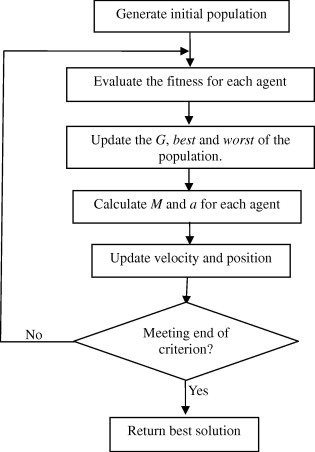
\includegraphics{images/GSA.jpg}
                \end{center}
                \caption{The Gravitational Search Algorithm}
            \end{wrapfigure}

            The equation of motion of a physical system completely determines its dynamics, as such, it the goal of us as physicists (at least during the reading of the investigation) to find the sequence positions that satisfy (i.e. solve) the equation of motion.  Analytically, the equation of motion is often a second-order differential equation, but we can still do out best to solve it on a computer.  There is a near infinite number of methods to approximating a solution to a differential equation (called \emph{numerical integrators}) using finite techniques, but here we use the so-called `symplectic Euler Method'

            \begin{align}
                v_n^i &= r_i v_{n-1}^i + a_{n - 1}^i \\
                x_n^i &= x_{n - 1}^i + v_n^i
            \end{align}

            where $x_n^i, v_n^i$ are the position and velocity, respectively, of mass $i$ at step $n$.
\clearpage
\pagebreak

        \section*{Branch \& Bound}

            There are two (unsurprising) core components to the Branch \& Bound method: \emph{Branch}, where the search space is recursively partitioned into subsets that could contain the optimizer, and \emph{Bound}, where each of these subsets is effectively represented by the lowest (i.e. bounding) fitness over all its candidate solutions.  With only branching, this method reduces to brute-force;  it is with the bounding consideration that the solution space can be more efficiently searched.  The Branch \& Bound method has been applied to the Traveling Sales Problem\cite{branch_bound}.  Psuedo-code for a generic Branch \& Bound is implemented in algorithm \ref{alg:bb}.

            The branching stage recursively partitions the search space into two or more, typically disjoint, subsets; this could be done with a $k$d-tree.  In actual applications of this method, a data structure must be used to store these subsets of candidate solutions; these structured sets are called \emph{instances}.  In other words, for a collection of solutions that have some relationship to each other $I$, there is the corresponding collection $S_I$ of solutions that \emph{do not} have a relationship to each other (i.e. a \emph{set}).  Some common choices for this structure are a: queue (First in, First out), stack (Last in, First out), and a priority queue (sorts the solutions by their fitness)\cite{Clausen2003BranchAB}.  Choosing a queue structure results in traversing the ``partitioned solutions space tree'' using a breadth-first search, a stack structure results in a depth-first search, and a priority-queue in a ``best-first search''\cite{toolbox}.

            The bounding stage of the algorithm takes each instance and calculates the lowest (assuming a minimization problem) fitness over all its elements (i.e. candidate solutions).  Then while traversing the tree, the bound of each node (i.e. the root of some subtree) is compared to a globally known bound defined as the least bound found so far.  If the current bound is greater than the global, the alogrithm does not proceed down the rest of that branch i.e. sub-tree as it cannot yield a better solution.

            \begin{algorithm}
                \DontPrintSemicolon
                \caption{Branch \& Bound}
                \label{alg:bb}
                \KwIn{problem, objective function $f$, lower bound function $bound$}
                \KwOut{solution}
                \tcp{initialize solution}
                $x \gets $ initial guess\;
                $B \gets f(x)$\;
                \tcp{initialize structure}
                $candidate\_structure \gets$ all candidate solutions of problem\;
                \tcp{traverse tree}
                \While{candidate\_structure is not empty}{
                    $node \gets candidate\_structure.pop()$\;
                    \eIf{node is a single solution and $f(node) < B$}{
                        $optimum \gets node$\;
                        $B \gets f(node)$\;
                        \tcp{otherwise node has multiple branches or it's worse}
                    }{
                        \For{branch in node}{
                            \If{$bound(branch) <= B$}{
                                $candidate\_structure.push(branch)$
                            }
                            \tcp{otherwise optimum isn't in branch}
                        }
                    }
                }
                \Return{optimum}
            \end{algorithm}

\pagebreak

    \section*{Results}

        The Gravitational Search Algorithm (GSA) has been benchmarked and compared to other methods such as Particle Swarm Optimization (PSO) and Real Genetic Algorithm (RGA)\cite{GSA}.  These data are done using unimodal (ref. \cite{GSA} table 1) and multimodal (ref. \cite{GSA} table 2) benchmarks in high dimenions ($n$) and multimodal benchmarks in low dimension (ref. \cite{GSA} table 3).

        Because GSA has great ``attractive power'', it should excel at optimizing unimodal functions.  Figure \ref{fig:unimodal} compares this attractive power against the other methods.

        \begin{figure}[h]
            \centering
            \includegraphics*[width=0.86\textwidth]{images/unimodal.png}
            \caption{High dimensional unimodal benchmarks of RGA, PSO, and GSA}
            \label{fig:unimodal}
        \end{figure}

        For high-dimensional multimodal benchmarks (figure \ref{fig:multimodalHigh}), GSA still performs decently well, but is not able to beat its counterparts for some benchmarks.  These data show that GSA is less effcicient at escaping local optima.  Since the considered multimodal benchmarks have an exponentially increasing number of local minima as the dimension grows, using GSA on even on many randomly chosen initial candidate solutions might still not yield a reasonably good optimum.

        \begin{figure}[h]
            \centering
            \includegraphics*[width=0.86\textwidth]{images/multimodal_variable_dimensions.png}
            \caption{High dimensional multimodal benchmarks of RGA, PSO, and GSA}
            \label{fig:multimodalHigh}
        \end{figure}

\pagebreak

        For low dimensional benchmarks (figure \ref{fig:multimodalLow}), all the considered methods perform similarly.

        \begin{figure}[h]
            \centering
            \includegraphics*[width=0.86\textwidth]{images/multimodal_fixed.png}
            \caption{Low dimensional multimodal benchmarks of RGA, PSO, and GSA}
            \label{fig:multimodalLow}
        \end{figure}

    \section*{Conclusion}

        Because the complexity of combinatorial optimization problems is such a wide spectrum, no single algorithm will be the perform the best for every problem.  For problems with small search spaces, exact methods such as Branch \& Bound are a good choice because they neccessarily find the global optimum, are straightforward to implement, and perform reasonably well.  For problems with either a larger search space or higher complexity, heuristic algorithms such as Gravitational Search should be considered because they are non-exhaustive and generally lead to reasonable performance in both run-time and optimization.  

    \printbibliography

\end{document}
